%----------------------------------------------------------------------------------------
%	PACKAGES AND OTHER DOCUMENT CONFIGURATIONS
%----------------------------------------------------------------------------------------

\documentclass[12pt]{report}
\usepackage[english]{babel}
\usepackage[utf8x]{inputenc}
\usepackage{amsmath}
\usepackage{graphicx}
\usepackage[colorinlistoftodos]{todonotes}
\usepackage{float}
\usepackage[margin=1in]{geometry}
\usepackage[toc,page]{appendix}
\usepackage{cleveref}
\usepackage{hyperref}
\usepackage{subcaption}
\usepackage{dsfont}


\begin{document}

\begin{titlepage}

\newcommand{\HRule}{\rule{\linewidth}{0.5mm}} % Defines a new command for the horizontal lines, change thickness here

\center % Center everything on the page
 
%----------------------------------------------------------------------------------------
%	HEADING SECTIONS
%----------------------------------------------------------------------------------------


\raisebox{-.2\height}{\includegraphics[width=180px, height=120px]{img/garde/logo_centrale.png}}%
\hfill
\raisebox{-.1\height}{\includegraphics[width=180px, height=60px]{img/garde/logo_dreem.png}}%
\\[2cm]

%----------------------------------------------------------------------------------------
%	TITLE SECTION
%----------------------------------------------------------------------------------------

\HRule \\[0.4cm]
{ \LARGE \bfseries Automatic sleep stages classification}\\[0.3cm] % Title of your document
{ \large End-of-studies internship}\\[0.3cm] % Title of your document
\HRule \\[1cm]
 
 %----------------------------------------------------------------------------------------
 %	DATE SECTION
 %----------------------------------------------------------------------------------------
 
 {\large 18 May - 22 November, 2015}\\[1cm] % Date, change the \today to a set date if you want to be precise
 
%----------------------------------------------------------------------------------------
%	PROMO SECTION
%----------------------------------------------------------------------------------------
  
\begin{minipage}{0.9\textwidth}
\begin{flushleft} \Large
\bfseries Promo 2014 % Promo
\end{flushleft}
\end{minipage}
\\[1cm]
 
%----------------------------------------------------------------------------------------
%	AUTHOR SECTION
%----------------------------------------------------------------------------------------
\normalsize \emph{Student:}\\
Clément \textsc{Nicolle} \\
\footnotesize Option Mathématiques Appliquées (OMA) - Majeure Data Science \\
\footnotesize Filière Métiers de la Recherche \\
\footnotesize Master Mathématiques, Vision, Apprentissage (MVA) - ENS Cachan
\\[1cm]

%----------------------------------------------------------------------------------------
%	TUTORS SECTION
%----------------------------------------------------------------------------------------
\begin{minipage}{0.5\textwidth}
\begin{flushleft} \normalsize
 \emph{School tutors:}\\
Option, Master: Nikos \textsc{Paragios} \\
Filière: Jean-Hubert \textsc{Schmitt}
\end{flushleft}
\end{minipage}
~
\begin{minipage}{0.4\textwidth}
\begin{flushright} \normalsize
\emph{Company supervisor:} \\
Mathieu \textsc{Galtier} % Supervisor's Name
\end{flushright}
\end{minipage}\\[2cm]

% If you don't want a supervisor, uncomment the two lines below and remove the section above
%\Large \emph{Author:}\\
%John \textsc{Smith}\\[3cm] % Your name


\vfill % Fill the rest of the page with whitespace

\end{titlepage}


\chapter*{Synthèse / Executive summary}
\addcontentsline{toc}{chapter}{Synthèse / Executive summary}
\section*{Synthèse}
\addcontentsline{toc}{section}{Synthèse}

L'annotation des états de sommeil n'est pas un problème simple dans la mesure où certaines phases sont très similaires. Deux médecins entre eux ne sont jamais parfaitement en accord. Son automatisation est néanmoins utile car l'annotation manuelle est coûteuse en temps.

Le bandeau Dreem permet l'acquisition d'électro-encéphalogrammes (EEG) à travers des électrodes frontales ainsi que de mouvements grâce à un accéléromètre. À partir de ces signaux, j'ai implémenté un algorithme de classification automatique des états de sommeil.

Il m'a d'abord fallu comprendre les aspects biologiques, neurologiques, du problème, afin d'extraire des signaux les informations les plus qualitatives possible. De plus, j'ai dû intégrer cette mission dans l'organisation de Dreem : depuis la conception du bandeau jusqu'à l'utilisateur final, il existe de nombreux maillons, et l'hypnogramme tient directement sa place dans la chaîne. J'ai notamment appris à réfléchir à des méthodes "Online", que l'on pourrait traduire par "à la volée", car, contrairement à tous les problèmes auxquels j'avais été confronté jusqu'alors, nous n'avons pas connaissance du signal futur au fur et à mesure de la nuit. J'ai également appris de nouveaux langages informatiques, notamment Django pour calculer et afficher des résultats sur notre serveur. Enfin, en parallèle de ces aspects techniques, j'ai eu la chance d'organiser un challenge de Data science, d'encadrer un séminaire de recherche ou encore de rédiger des articles de blog.

Mais le contenu scientifique directement lié à l'algorithme de classification des états de sommeil a occupé la plus claire partie de mon stage.

J'ai beaucoup travaillé à l'extraction de features. Il était notamment utile, pour améliorer notre compréhension sur le sommeil aussi bien que pour nourrir mon algorithme, de développer des détecteurs de différents phénomènes nocturnes cérébraux. Toutes les features implémentées ont été optimisées, testées, comparées, pour retenir finalement une modèle de dimension 29.

Différents classifieurs, que j'avais pour la plupart étudiés en cours mais qui ont été adaptés à ce problème particulier, ont été confrontés. En fin de compte, la Random Forest a permis d'obtenir les meilleurs résultats.

Finalement, les niveaux de performance obtenus sont de l'ordre de grandeur de l'état de l'art, la comparaison ayant été faite avec des problèmes qui se rapprochent au maximum du notre. L'hypnogramme sera présent sur la version bêta du bandeau Dreem, prévue pour début 2016.

\newpage
\section*{Executive summary}
\addcontentsline{toc}{section}{Executive summary}

Sleep stages annotation is a difficult problem as some phases are hard to distinguish. Two doctors indeed relatively disagree between each others. Making it automatic, however, is necessary because manual scoring is time-consuming.

Dreem headband acquires electroencephalogram (EEG) signals through electrodes placed on the forehead of the sleeper as well as movements thanks to an accelerometer. From these signals, I implemented an automatic classification algorithm for sleep stages.

I first needed to understand neurological aspects of the problem, in order to be able to extract qualitative informations from the signals. In addition, it was important to place this mission in the context of the company: from headband conception to the final user, there is a series of links and the hypnogram is one of them. For example, I learned to think the "Online" way, because, contrary to the problems I had to face so far, we have no knowledge of future signal through the night. I also learned new computer languages, such as Django in order to compute and display results on our server. Eventually, in parallel with those technical aspects, I had the opportunity to organize a Data science challenge, to supervise a research seminar or to redact blog articles.

Nevertheless, scientific content directly linked to the classification algorithm represented the major part of my internship.

I worked a lot on features extraction. It was useful, notably, in order to gain a better comprehension of sleep as well as to feed my algorithm, to develop detectors for the different physiological phenomenons that occur in the brain during the night. All the implemented features have been tuned, tested, evaluated, and resulted in a 29-dimensional model.

Different classifiers, most of them I had studied during courses but that have been adapted to this particular problem, were confronted. Finally, Random Forest gave the best results.

The obtained performance levels were of the same order of magnitude of state-of-the-art on similar problems. The hypnogram will be present on the beta version of Dreem headband to be released in the beginning of 2016.

\newpage
  \tableofcontents
\newpage

\chapter*{Motivation}
\addcontentsline{toc}{chapter}{Motivation}

Neurology is one of the most studied topic in science nowadays. It has the particularity to be at the crossroads of various fields such as medicine, biology, mathematics or computer science (\cite{bear2007neuroscience}). In this context, Dreem's ambition is to bring neuroscientific advances to people. This is what motivated me to join the adventure in its scientific aspect.

In a first part of its development, Dreem focused on sleep. Sleep constitutes an important proportion of brain activity, and yet few importance seems to be brought on it. On one side, we spend a third of our life sleeping. Different mechanisms, that concern memory, cognitive aptitudes or energy regeneration, take place while sleeping (\cite{carskadon2000normal}). On the other side, it is rare to interrogate ourselves about the way we sleep and our night habits (\cite{ohayon2000prevalence}).

Based on a discovery by Ngo in 2013 (\cite{ngo2013auditory}), Dreem is conceiving an active headband to improve the quality of sleep, and particularly deep sleep. But it also aims to furnish clear and preprocessed informations about his nights to the user, in order to have him improving his comprehension of brain and his habits. In that measure, we asked ourselves about the optimal way to represent a night and display it to the future users.

In 2007, AASM established 5 synthetic categories (\cite{berry2012aasm}), or sleep stages, that happen during the night. The evolution of this stages along time is the most common way to represent a night, and is called an hypnogram.

Different personal sleep trackers have been available in those recent times: apps (Sleep Genius, SleepCycle, SleepBot, Sleep Time...), wristband (Jawbone, Fitbit, Basis...), smart-watches (Activité by Withings, iWatch by Apple...), bed-based monitory systems (Beddit, Misfit, Withings Aura...). After testing some of them (Sleep Genius, Jawbone, Fitbit and Withings Aura), we quickly realize that the displayed hypnograms are quite different, in addition of being incomplete, with often 3 sleep stages proposed instead of 5.

Indeed, sleep phenomenons occur for a major part in the brain. Dreem's headband's electrodes allow to directly access to brain signals and it then should result in more accurate hypnograms compared with the ones doctors score. An accelerometer is also present on the headband.

My internship has consisted in implementing an automatic hypnogram based on data acquired through Dreem headband.

To achieve this goal, I had to go through different aspects.

On the one hand, my understanding of what sleep is and what an hypnogram is, of the usage we wished to make of it, as well as the way of implementing it as part of Dreem organization, was primordial. I had the opportunity to tackle different issues in different domains here: neuroscience and biology, marketing, management, computer science or redaction.

On the other hand, I mainly focused on the scientific, mathematical implementation of an automatic sleep-stage classifier. A huge amount of my time was dedicated to exploring different possible features. After processing my database, I was able to test various classification algorithms. An appropriate metrics for the problem was used to compare their performances. Finally, I selected a final version to be compared with other research publications, and developed the whole infrastructure for hypnograms at Dreem.

\chapter{Context and organisation}

In this chapter, I explain the context of my internship at Dreem, present my missions and the way I got organized. 

\section{Brief history}

\subsection{The company}

Dreem is a start-up company started in July 2014 in Paris, with another office in San Francisco. Today, it counts 30 employees.

Dreem aims to valorize neuroscience and create products and services based on scientific advances. Concretely, inspired from \cite{ngo2013auditory}, we are developing the first active wearable product that increases the quality of deep sleep by using audio stimulations synchronized with brain activity.

A lot of research work is made in the fields of machine learning and neuroscience, but also for designing the product and embed the algorithms. We are still in a prototyping stage. Each day, between 5 and 10 headbands leave the office to be worn during the night, and our database keep increasing this way for the moment. The next important step will be the release of a beta version in the beginning of next year.

\subsection{Dreem headband}

Dreem headband is composed of three arches as you can see on \ref{fig:me_headband}. We use dry electrodes on the forehead in order to acquire electroencephalogram (EEG) signal. The hardware materials, along with embedded algorithms, are placed on the arch above the head. There is also an accelerometer to track movements.

Piezoelectric components above the ears emit sounds stimulations in the correct stage of sleep, at the appropriate moment. The effects of these stimulations is to improve the quality of our deep sleep, which is important in term of memory and cognitive aptitudes as explain in \cite{mangold1955effects} or \cite{maquet2001role}

\begin{figure}[H]
\centering
\includegraphics[width=0.5\textwidth]{img/chap1/me_headband.png}
\caption{\label{fig:me_headband}Dreem headband}
\end{figure}

\subsection{Past research seminar}

During my third year at Centrale, I realized with a friend my research seminar of Applied Mathematics Option (OMA) at Dreem.

At that time, Dreem was just starting to record EEG with the headband, and, then, did not dispose of a lot of data. Hence we decided to work on a public database. It was composed of 30 annotated nights. Nevertheless, we decided to work on a unsupervised way. We looked at window of 30 seconds of signals and apply features extraction and clustering algorithms in order to determine if we could discriminate naturally the data points to fall back on the doctors' annotations.

I will not expand more on this project in the present report. At the end, we reached a maximum of 56,9\% matching between our predicted labels and neurologists' annotations, using a Hidden Markov Model presented in \cite{PGM}. This work mainly brought Dreem to know original features to analyze sleep EEG and put at their disposal a Python infrastructure in order to compare different features and algorithms between each others.

Feelings after this seminar were rather enthusiastic, as well from the school, Dreem, and my own point of view. I really enjoyed working here, as much for the content as for the environment, and was aware of the potential development of our project. Therefore, in January, I announced my wish to continue with Dreem, and was delighted that they welcome me for my end-of-studies internship.

\section{Place in the company}

In order to understand the role I play in the company and the interactions I have with my colleagues, I think it is important to present in a simplified way Dreem organization.

Apart from the direction and the marketing teams, we can consider that there exists 5 poles in the chains of Dreem headband conception:

\begin{itemize}
\item \textbf{Ergonomics / Design:} They are in charge of conceiving the headband's supports, the prototypes as well as the soon-to-be industrialized ones.
\item \textbf{Hardware:} Hardware pole is responsible for all the electronic acquisition of EEG.
\item \textbf{Embedded:} The embedded team communicates between the hardware and the algorithms. They notably traduce the Python code in C in order to embed it on a CPU in the headband.
\item \textbf{Algo / Neuro:} This is the team in which I work, hence I will be more accurate here. We are basically a group of 7 permanent persons. Mathieu is the director of our pole, also called R\&D. Three students have just started their thesis.

We are in charge together of the treatment and analysis of EEG signals. It requires abalities in machine learning, but also in neuroscience. We also try, then, to maintain a scientific background at the crossroads between mathematics, informatics, biology and medicine.

\item \textbf{Software / App:} They take care of the website as well as of our server where nights are stored and analyzed. They are also conceiving the mobile app where our users could find all the relevant informations in order to understand and improve the way they sleep. These features might be sleep reports, white noise generator or EEG visualization.

\end{itemize}

A representation of the pipeline from raw materials to abstract data can be found on figure \ref{fig:teams}.

\begin{figure}[H]
\centering
\includegraphics[width=1\textwidth]{img/chap1/teams.png}
\caption{\label{fig:teams}Schematic Dreem's organisation}
\end{figure}

\section{Missions}

My principal task was the creation of an infrastructure for automatic sleep stages classification. Though, to achieve this goal, I had to cope with different missions:

\begin{itemize}
\item \textbf{Brain comprehension:} In order to be able to extract high-level features from EEG signals, I had to gain a good comprehension of brain, EEG and sleep. Then I went through a lot of readings on the topics as well as discussions with experts. Dreem is now part of European Human Brain Project. We have regular discussions with other researchers involved in the project.
\item \textbf{Machine Learning algorithms:} This was the main reason why I have joined Dreem project. I had to develop optimal algorithms able to score nights accurately. The framework used at Dreem is Python, that I had the chance to already know. Nevertheless, I had largely time to explore it deeper in order to implement the whole pipeline from raw signal to hypnogram.
\item \textbf{Server infrastructure:} This task was executed in cooperation with Software pole. I had to learn Django language, a framework web for Python, in order to implement the results of my algorithms on our server, also called back-end. On this server, when a new night is uploaded, algorithms are run automatically, and we can quickly have a look at the displayed results.
\item \textbf{Embedded algorithms:} This task was in cooperation with Embedded pole. One of the role of embedded team is to translate our Python code to C in order to put it on a CPU on the headband. Hence, we implemented matching metrics to check if the results obtained in the embedded CPU is the same as the results we got previously in Python. 
\item \textbf{MVA challenge:} Last year, Dreem proposed a MVA challenge. I went through the best reports to grab ideas for my own problem. Furthermore, we revealed this year a new challenge based on sleep stages classification. It will be a way to get new ideas, but also a leverage to make Dreem known and for recruitment.
\item \textbf{OMA research seminar:} After realizing myself my seminar at Dreem, we welcome this year two third-year students. I am in charge of the supervision of the project, which consists in developing metrics and later on a clustering infrastructure on hypnograms. The first phase has begun with theoretical researches about dimensionality reduction and clustering algorithms on temporal data points.
\item \textbf{Blog vulgarisation articles:} I also wrote blog articles to give a simplified view of our scientific work to future users.
\end{itemize}

\begin{figure}[H]
\centering
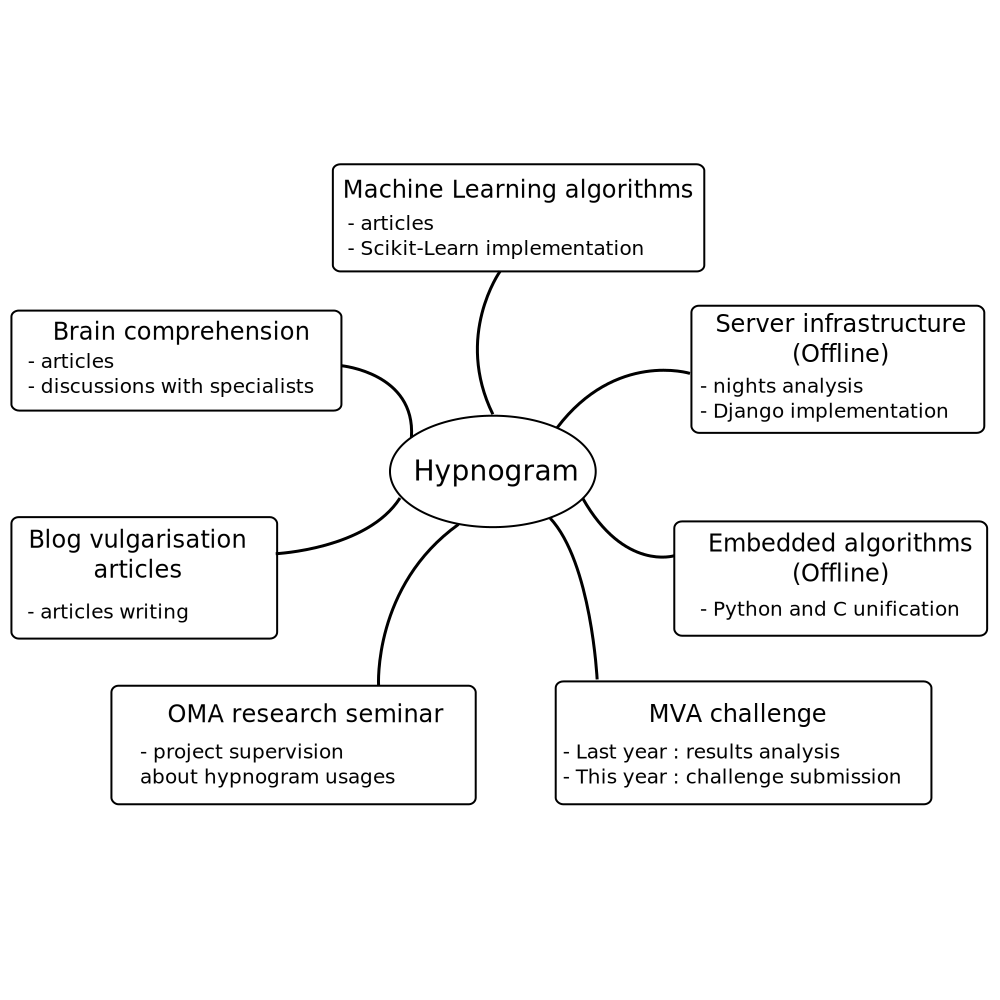
\includegraphics[width=1\textwidth]{img/chap1/missions.png}
\caption{\label{fig:missions}My missions}
\end{figure}

\section{Offline vs Online} \label{chap:Offline vs Online}

One of the novelty I had to face during my internship was the implementation of Online algorithms, to be compared with Offline ones.

\subsection{Offline algorithms}

During my studies, I always treated the Offline case. As a matter of fact, for school projects, we always dispose directly of the whole dataset. Hence we have a global view on it, and no limitation on algorithms to run.

As far as Dreem is concerned, we can run Offline algorithms on a night only when it is uploaded on our server, or on a set of nights already recorded. This is why I learned Django for. I can here compute a more complete version of the hypnogram than the Online one that we will now examine.

\subsection{Online algorithms}

On the other hand, we have some constraints on the algorithms to run on the headband:
\begin{itemize}
\item We do not know the future. Data are acquired point by point, and hence we only can use features and algorithms that do not take into account the end of the night. It supposed a twist in the way of thinking computations. For the hypnogram, I had to think this way, as we wish the user could observe a summary of his night on his smartphone just after waking up. Contrary to the server, all the computations are here embedded.
\item We need fast and low-energy-consuming algorithms. As a matter of fact, battery usage is a crucial point for Dreem headband. We need it to last at least a night of course, but even two or three for more comfort.
\end{itemize}

Taking into account those parameters, we conceived the pipeline for the Online algorithms.

\begin{figure}[H]
\centering
\includegraphics[width=1\textwidth]{img/chap1/online_archi.png}
\caption{\label{fig:online_archi}Online algorithms architecture}
\end{figure}

The acquired EEG signals are fist filtered to eliminate notably 50 Hz frequency, corresponding to European electrical network. A machine learning algorithm then eliminate the parts of not-sufficient quality. The Combiner block generates a single signal from the multiple electrodes. We use this signal to generate the stimulations and also the hypnogram.

I particularly work on the part circled in red. The role of the Analyzer is to compute all the features and then the classification algorithm, that we will analyze in details in chapter \ref{chap:Scientific work}, to obtain the hypnogram, internally called "Dreemnogram".

The role of the enabler is to detect the moments when we allow stimulations. It directly uses the sleep stages classification resulting from Dreemnogram. Then the stimulator determines the accurate time to stimulate the sleeper.

\section{Internship proceedings}

We can approximately divide the way I worked in two phases: research and production.

\begin{itemize}
\item It took me first a few weeks to immerse into the topic, grab an overview of scientific works in the domain of automatic sleep stages classification, establish a review of the state-of-art. I then explored the different possible features. Some of them were directly inspired from articles, other tried to be more innovative. After computing a solid base of features, I implemented the different classification algorithms. I determined a metrics in order to compare my results, and mostly used the knowledge acquired during my last year of studies for the algorithms.

Furthermore, I kept having discussions about neuroscience with external researchers and about machine learning with my team and teams from other start-ups.

\item Of course, during this research period, I did not stay in the purely theoretical sphere. All the features were implemented in Python, with two versions, Offline and Online (\ref{chap:Offline vs Online}). Then it took me some time to run the classifiers, optimize their parameters, and display the resulting hypnograms on our server as well as working with the embedded team to put it inside the headband.

We put in place at Dreem, for this more productive work, a management method called "Agile". A known tool that helps for this is "Jira". Agile method consists in phases of one or two weeks of work, divided in different elementary tasks, in order to achieve a final accomplished goal. It is an interesting way to focus on results after having explored the ways to reach them optimally.
\end{itemize}


\chapter{Scientific work} \label{chap:Scientific work}

In this chapter, I present the pipeline of the automatic sleep stages classifier achieved during my internship.

\section{Problem position}

\subsection{Data}

Electroencephalogram (EEG) detects the electrical activity of the brain by using small metal discs called electrodes. Brain cells emit electrical impulses and stay active even when sleeping. Depending on their position on skull, we can observe different phenomenons. On Dreem headband, we acquire brain EEG on the forehead of the sleeper.

The data on which I worked are recordings of EEG obtained through Dreem headband. They are sampled at 250 Hz, and measured in micro-volts. The amount of records kept increasing during my internship. My first database was quite small, but, at the end, I could use almost 800 hours of signals corresponding to 121 different nights.

A raw EEG needs to be preprocessed in order to gain some comprehension of it. As a matter of fact, on raw signals, the power around frequency 50 Hz is huge for example, as it corresponds to French electrical network. Moreover, artifacts can be present, as well as phases of poor quality due to bad electrodes materials or imperfect adherence with the skin.

For these reasons, we only work on frequencies below 18 Hz, as they are the ones interesting for sleep as we will see in the next part. We removed the moment of bad quality by using an algorithm made by a colleague, who manually labeled epochs of bad quality and then identified it using a Random Forest algorithm (see \ref{section:Random Forest} for more information).

Table \ref{fig:eeg_30s} shows an example of 30 seconds of EEG:

\begin{figure}[H]
\centering
\includegraphics[width=1\textwidth]{img/chap2/eeg_30s.png}
\caption{\label{fig:eeg_30s}30 seconds of EEG}
\end{figure}

In addition with EEG signals, I also had at my disposal an accelerometer, sampled at 250 Hz too for the moment. It is placed on the arch above the skull. The resulting signals are indeed integrated, and correspond to the relative position along the three space directions.

On table \ref{fig:acc_night} are represented the coordinates of the accelerometer vector for a record of 3 hours and 42 minutes.

\begin{figure}[H]
\centering
\includegraphics[width=1\textwidth]{img/chap2/acc_night.png}
\caption{\label{fig:acc_night}Accelerometer coordinates over a record of 3 hours and 42 minutes}
\end{figure}

\subsection{Hypnogram, what is it exactly ?}

It is generally known that there exists different phases of sleep. The first categorization was made back in 1968 by Rechtschaffen and Kales (\cite{rechtschaffen1968manual}). At that time, they considered 6 stages. It was reviewed in 2007 by the American Academy of Sleep Medicine (AASM), which basically merged two stages and established then their number to 5, with rules to determine it (\cite{berry2012aasm}).

According to the AASM, the different stages of sleep are:
\begin{itemize}
	\item \textbf{Wakefulness:} We are aware of our environment. We can observe beta waves (irregular, low intensity, fast frequency), and more and more alpha waves (regular, moderate intensity, 8-12 Hz) as we start to relax.
	\item \textbf{N1:} Commonly referred to as somnolence. Muscles are still active and we can be easily awaken. It is characterized by alpha and theta waves (4-8 Hz).
	\item \textbf{N2:} Around half of our nights is spent in this intermediate stage. It is characterized by the raise of isolated high-amplitude delta wave (< 4 Hz), generally at 1 Hz, called K-complex. It is usually followed by bursting oscillations at 12-14 Hz lasting 0.5 to 2 seconds, called spindles.
	\item \textbf{N3:} Also known as "deep sleep". In this stage, we state an absence of reaction to stimuli. It is composed of a succession of delta waves, also said slow oscillations. During this stage, what we have learned during the day is transfered to our declarative memory (concepts, words, ideas, facts...). This is a crucial epoch for Dreem as the goal of the headband is to stimulate at slow oscillations in order to strengthen in and then gain better cognitive and memory aptitudes.
	\item \textbf{Rapid Eye Movement (REM):} Publicly known as "paradoxical sleep", this is the time when the majority of dreams happen. Muscles are paralyzed, but an electro-oculogram would show eye movements, hence the name REM. This stage strengthens our procedural memory, which corresponds to movements. 
\end{itemize}

We find in \cite{moorcroft2003understanding} a relevant table in order to understand the differences between sleep stages: 

\begin{figure}[H]
\centering
\includegraphics[width=0.5\textwidth]{img/chap2/stages.png}
\caption{\label{fig:stages}EEG, EOG, and EMG characteristics of each stage of sleep. The most important aspects for determination of each stage are shown darker than the less important aspects}
\end{figure}

It points out that we normally use different indicators to know sleep: brain (EEG), eyes (EOG) and muscles (EMG). Actually, complete analysis of sleep usually requires a full set of metrics, called polysomnograph, which also takes into account heart rate (ECG) or temperature.

Nevertheless, at Dreem, we only disposed of the EEG obtained with a few electrodes on the forehead (to be compared with a full set of electrodes all around the head for polysomnograph) at diverse quality, and an accelerometer.

To finish, an hypnogram is simply the evolution of sleep stage during the night. 

\begin{figure}[H]
\centering
\includegraphics[width=0.8\textwidth]{img/chap2/hypno_net.png}
\caption{\label{fig:hypno_net}Typical hypnogram}
\end{figure}

A typical night is generally composed of three to five cycles of 60 to 90 minutes. A cycle starts with wakefulness or a light phase of sleep, and then goes deeper, to potentially finish in REM. We generally observe N3 sleep in the first half of the night and REM in the second.

\subsection{Concretely, how do we obtain an hypnogram ?}

To obtain an hypnogram, you need a doctor specialized in sleep. He looks at windows of 30 seconds of a polysomnograph (according to the data he gets at his disposal) and, according to the AASM rules, is able to determine the corresponding stage.

One important aspect here is that they may be no ground truth for a given window. REM and Wake, or N1, for instance, are quite difficult to differentiate if we only have an EEG. Indeed, it is explained in \cite{basner2008inter} that, if we present isolated 30-second windows to different doctors, they will agree by mean at around 80\%. Of course, this rate can be improved if they can follow the evolution of the night, and have a vision of the night before and after the considered window.

At Dreem, concretely, we got our own doctor, Eden, labeled our nights. At the time I am writing this report, she went through 121 different nights acquired with Dreem headband. We implemented our own scoring infrastructure to allow her to label the nights. This labeled windows constitute the database of my model.

\newpage
\section{Features extraction}

In this chapter, we will explore the different features I implemented. In order to compare the features between each others, we will consider the three windows taken in different sleep stages of table \ref{fig:3windows}.

\begin{figure}[H]
\begin{subfigure}{1.\textwidth}
	\centering
	\includegraphics[width=0.5\textwidth]{img/chap2/wake_window.png}
	\caption{Wake}
	\label{fig:wake_window}
\end{subfigure}

\begin{subfigure}{1.\textwidth}
	\centering
	\includegraphics[width=0.5\textwidth]{img/chap2/n2_window.png}
	\caption{N2}
	\label{fig:n2_window}
\end{subfigure}

\begin{subfigure}{1.\textwidth}
	\centering
	\includegraphics[width=0.5\textwidth]{img/chap2/n3_window.png}
	\caption{N3}
	\label{fig:n3_window}
\end{subfigure}

\caption{\label{fig:3windows}Three 30-second of EEG signal, respectively in Wake, N2 or N3 stage}
\end{figure}

The windows were voluntarily taken relatively far from each others.

With naked eye, we observe in wake high-frequency irregular oscillations. In the N2 window, we identify a K-complex and some spindles around. We find typical delta waves in N3.

\subsection{Spectral approach}

As pointed out when defining the different stages of sleep, brain waves play a primordial role in differentiating stages. Then it is logical to adopt first a spectral analysis for EEG. There exists two major methods: Fourier and Wavelets.

\subsubsection{Fast Fourier Transform} \label{subsubsection:Fourier}

Fourier Transform may be the most famous method to decompose a signal. It consists in a switch from time domain, with no frequency information, to frequency domain, but without time information. Concretely, a convolution with an orthonormal basis of sine and cosine functions is computed to obtain coefficients corresponding to the different frequencies . The theoretical details are recovered in appendix \ref{chap:Fourier}.

In practice, we compute a discrete Fourier transform over our sampled points. Whereas a naive implementation would give a complexity in $O(n^2)$, a clever implementation, Fast Fourier Transform (FFT), using "divide and conquer" principle, allows for a mean complexity of $O(n\log(n))$ (\cite{walker1996fast}). I used the Python package numpy to compute the FFT.

Along a window of 30 seconds of 1D-signal, just as EEG, we can compute a spectrogram. This is the 3D representation, using color scale, of the evolution of the power spectral densities corresponding to different frequency bins over the signal. In our case, since each window contains 7,500 points sampled at 250 Hz, the Nyquist-Shannon sampling theorem allows to compute 7,500 Fourier coefficients, between 0 and 125 Hz. As EEG is a real signal, Fourier coefficients are symmetric: we only keep half of them.

Furthermore, frequencies over 18 Hz play a minor role in sleep characterization. Hence, I focused on frequencies below 18 Hz.

For our three illustrative windows in figure \ref{fig:3windows}, the Fourier coefficients and spectrograms are displayed in figure \ref{fig:3winsows_fft}).

\begin{figure}[H]
\begin{subfigure}{0.5\textwidth}
	\centering
	\includegraphics[width=1\textwidth]{img/chap2/wake_fft.png}
	\caption{Wake}
	\label{fig:wake_fft}
\end{subfigure}
\begin{subfigure}{0.5\textwidth}
	\centering
	\includegraphics[width=1\textwidth]{img/chap2/n2_fft.png}
	\caption{N2}
	\label{fig:n2_fft}
\end{subfigure}

\begin{subfigure}{1.\textwidth}
	\centering
	\includegraphics[width=0.5\textwidth]{img/chap2/n3_fft.png}
	\caption{N3}
	\label{fig:n3_fft}
\end{subfigure}

\caption{\label{fig:3winsows_fft}Raw signal, Fourier coefficients and Spectrogram for Wake, N2 and N3 windows}
\end{figure}

We can briefly observe that Wake has general higher frequencies large Fourier coefficients. The peak around 12 Hz for N2 corresponds to spindles. For N3, slow oscillations may be deduced from the spectrogram by the dark red bands in the lower part.

In order to get accurate features, I used our knowledge on sleep waves. Basically, sleep waves and their frequencies are the following:

\begin{table}[H]
\centering
\begin{tabular}{c|c}
Waves & Frequencies range \\\hline
Delta ($\delta$) & 0.5 - 4 Hz \\
Theta ($\theta$) & 4 - 8 Hz \\
Low frequencies ($\delta+\theta$) & 0.5 - 8 Hz \\
Alpha ($\alpha$) & 8 - 12 Hz \\
Sigma ($\sigma$) & 11 - 15 Hz \\
Beta ($\beta$) & 15 - 30 Hz \\
K-complex ($K$) & 0.9 - 1.1 Hz \\
\end{tabular}
\caption{\label{tab:waves_freq}Sleep brain waves and corresponding frequencies range}
\end{table}

From this and after different tuning, the different features I kept for my final algorithm were:
\begin{itemize}
\item \textbf{Band powers:} Power spectral density corresponds to the square of the modulus of Fourier coefficients. I computed it in the 7 defined frequencies ranges. In addition, I added the relative power of these different bands, by dividing the power in a range by the overall spectral power.
\item \textbf{Spectral edges:} For a given ratio $r$, it corresponds to the frequency such that, by integrating the power spectral density from 0 to this frequency, we reach $r$\% of the total spectral power. I used 3 different values for $r$: 50\% (Spectral Centroid, or SC), 90\% (SEF90) and 95\% (SEF95).
\end{itemize}

Hence 16 resulting coefficients: $\delta$, $\theta$, $\delta+\theta$, $\alpha$, $\sigma$, $\beta$, $K$, $\delta_r$, $\theta_r$, $\alpha_r$, $\sigma_r$, $\beta_r$, $K_r$, $SC$, $SEF90$ and $SEF95$.

Finally, the resulting values for our 3 illustrative windows are:
\begin{table}[H]
\centering
\scalebox{0.6}{
\begin{tabular}{|l|r|r|r|r|r|r|r|r|r|r|r|r|r|r|r|r|}
\hline
\multicolumn{1}{|c|}{} & \multicolumn{1}{c|}{$\delta$} & \multicolumn{1}{c|}{$\theta$} & \multicolumn{1}{c|}{$\alpha$} & \multicolumn{1}{c|}{$\sigma$} & \multicolumn{1}{c|}{$\beta$} & \multicolumn{1}{c|}{$K$} & \multicolumn{1}{c|}{$\delta+\theta$} & \multicolumn{1}{c|}{$\delta_r$} & \multicolumn{1}{c|}{$\theta_r$} & \multicolumn{1}{c|}{$\alpha_r$} & \multicolumn{1}{c|}{$\sigma_r$} & \multicolumn{1}{c|}{$\beta_r$} & \multicolumn{1}{c|}{$K_r$} & \multicolumn{1}{c|}{$SC$} & \multicolumn{1}{c|}{$SF90$} & \multicolumn{1}{c|}{$SF95$} \\ \hline
Wake & 2.67e9 & 1.44e9 & 2.54e8 & 1.98e7 & 6.13e5 & 2.06e8 & 4.11e9 & 4.50e-1               & 2.42e-1 & 4.27e-2 & 3.34e-3 & 1.03e-4 & 3.47e-2 & 1.18 & 6.55 & 7.77  \\ \hline
N2 & 2.92e8 & 1.42e8 & 2.99e6 & 1.87e5 & 6.71e4 & 4.53e8 & 4.34e8 & 4.56e-1 & 2.22e-1 & 4.69e-3 & 2.92e-4 & 1.05e-4 & 7.09e-2 & 1.05 & 5.87 & 6.08 \\ \hline
N3 & 4.33e9 & 1.97e8 & 3.11e6 & 1.196e5 & 1.13e4 & 3.22e8 & 4.53e9 & 5.56e-1 & 2.53e-2 & 3.99e-4 & 1.53e-05 & 1.45e-06 & 4.14e-2 & 7.33e-1 & 1.28 & 2.43\\ \hline
\end{tabular}
}
\caption{\label{tab:fft_val}Spectral features for Wake, N2 and N3 windows}
\end{table}

We observe spectral power densities globally higher in Wake. In N3, we can identify a predominance for slow waves.

\subsubsection{Wavelets transform}

Wavelet transform is an other, more modern time-frequency transformation. I will not detail the theory developed in \cite{mallat1999wavelet}, but the main difference with Fourier transform is that it adds a notion of locality. To say it an other way, while Fourier transform tells what frequencies in which amount is present in the signal, Wavelet transform tells what frequencies is present and where.

Instead of a spectrogram, we obtain a scalogram, giving more local informations.

\begin{figure}[H]
\begin{subfigure}{0.3\textwidth}
	\centering
	\includegraphics[width=1\textwidth]{img/chap2/wake_wavelets.png}
	\caption{Wake}
	\label{fig:wake_wav}
\end{subfigure}
\begin{subfigure}{0.3\textwidth}
	\centering
	\includegraphics[width=1\textwidth]{img/chap2/n2_wavelets.png}
	\caption{N2}
	\label{fig:n2_wav}
\end{subfigure}
\begin{subfigure}{0.3\textwidth}
	\centering
	\includegraphics[width=1\textwidth]{img/chap2/n3_wavelets.png}
	\caption{N3}
	\label{fig:n3_wav}
\end{subfigure}

\caption{\label{fig:3winsows_wav}Scalogram using Morlet wavelets for Wake, N2 and N3 windows}
\end{figure}

We can identify more clearly the slow oscillations for N3, the K-complex for N2.

I wanted to precise in this report that we have explored wavelets applications, nevertheless we decided not to implement it at Dreem for the moment, for several reasons:

\begin{itemize}
\item First because it requires more efforts to be developed in C to embed it in the headband.
\item We do not need it for compression as the single virtual channel we construct from the electrodes is small enough to be sent by Bluetooth on a smartphone.
\item The complexity to obtain coefficients in low frequencies bands is the same as for FFT, $O(n\log(n))$.
\item FFT features revealed sufficient in term of performance.
\end{itemize}

\subsection{Quantitative EEG features}

During my OMA seminar and, later on, my internship, I explored different proper-EEG features. The two kept for the final version of my algorithm was Petrosian Fractal Dimension and Detrended Flucutaion Analysis.

\subsubsection{Petrosian Fractal Dimension}

Pectrosian Fractal Dimension (PFD) is a method for computing the fractal dimension of a signal (\cite{esteller2001comparison}). The computation is detailed in appendix \ref{section:Petrosian Fractal Dimension}. It is a statistical index of complexity for EEG signal. The more the signal is "complicated", the higher PFD value is.

For our three illustrative windows, the PFD values are reported in table \ref{tab:pfd}.

\begin{table}[H]
\centering
\begin{tabular}{c|c}
Stage & PFD coefficient \\\hline
Wake & 1 + 2.35e-3 \\
N2 & 1 + 1.94e-3 \\
N3 & 1 + 8.46e-4 \\
\end{tabular}
\caption{\label{tab:pfd}Petrosian Fractal Dimension coefficient for Wake, N2 and N3 windows}
\end{table}

\subsubsection{Detrended Fluctuation Analysis}

Detrended Fluctuation Analysis (DFA) is more complex, in terms of computation as well as in terms of interpretation (\cite{morariu2007detrended}). The idea is to measure the extent of long-range correlations within a time series. A value of $1/2$ corresponds to uncorrelated white noise, a value of $1$ to pink noise or 1/f-noise, while a value around $3/2$ corresponds to a Brownian motion. Details may be found in appendix \ref{section:Detrended Fluctuation Analysis}.

For our three illustrative windows, the DFA values are reported in table \ref{tab:dfa}.

\begin{table}[H]
\centering
\begin{tabular}{c|c}
Stage & DFA coefficient \\\hline
Wake & 5.91e-1 \\
N2 & 9.01e-1 \\
N3 & 1.03 \\
\end{tabular}
\caption{\label{tab:dfa}Detrended Fluctuation Analysis coefficient for Wake, N2 and N3 windows}
\end{table}

\subsection{Sleep patterns detectors}

I present here the detectors implemented for some phenomenons occurring when sleeping: slow oscillations, spindles and alpha waves, and movements.

\subsubsection{Slow oscillations detector}

Slow oscillations occur particularly in N3 sleep, and correspond to the phenomenons Dreem headband wishes to emphasize. 

Different attempts were made to detect it, but we stay for the moment on a basics version using thresholds. A method using machine learning should soon be released. For the moment, we employ amplitude and temporal threshold in order to determine, possibly Online, whether we have a slow oscillation. The threshold are resumed on figure \ref{fig:so_detect}.

\begin{figure}[H]
\centering
\includegraphics[width=0.5\textwidth]{img/chap2/so_detect.png}
\caption{\label{fig:so_detect}Thresholds for Slow Oscillation detector}
\end{figure}

Figure \ref{fig:3windows_so} shows slow oscillations detected on our three illustrative windows.

\begin{figure}[H]
\begin{subfigure}{1.\textwidth}
	\centering
	\includegraphics[width=0.5\textwidth]{img/chap2/wake_sob.png}
	\caption{Wake}
	\label{fig:wake_window_so}
\end{subfigure}

\begin{subfigure}{1.\textwidth}
	\centering
	\includegraphics[width=0.5\textwidth]{img/chap2/n2_sob.png}
	\caption{N2}
	\label{fig:n2_window_so}
\end{subfigure}

\begin{subfigure}{1.\textwidth}
	\centering
	\includegraphics[width=0.5\textwidth]{img/chap2/n3_sob.png}
	\caption{N3}
	\label{fig:n3_window_so}
\end{subfigure}

\caption{\label{fig:3windows_so}Slow oscillations detection results in Wake, N2 or N3 stage}
\end{figure}

As expected, we mainly get it in N3. The isolated slow oscillation in N2 is a K-complex.

For a given window, slow oscillations features consist of the number, duration and amplitude of slow oscillations.


\subsubsection{Spindles and alpha waves detectors}

This is where I dedicated most of my times as far as features research is concerned.

Inspired from different articles, three methods were benchmarked:
\begin{itemize}
\item \textbf{Band pass and signal envelope algorithm, from \cite{ferrarelli2007reduced} and improved in \cite{astill2014sleep}}

We first apply a band-pass filter 11-16 Hz to the signal, and then look at the envelope of the resulting signal. Two amplitude threshold, $t_1$ and $t_2$ with $t_1 < t_2$, are set according to the mean envelope amplitude. A spindle is detected when the envelope of the filtered signal exceeds $t_2$ and then falls below $t_1$, and acknowledged if the corresponding duration falls between 0.3 and 3 seconds.

\item \textbf{Band pass Root Mean Square (RMS) overlapping moving windows, from \cite{molle2002grouping}}

We also apply a band-pass filtering at 11-16 Hz to the signal, but then look at the RMS value over windows of 0.1 second overlapping at 50\%. A spindle is detected if the RMS value exceeds an amplitude threshold set at twice the standard deviation of the filtered signal, and if its corresponding duration is between 0.3 and 3 seconds.

\item \textbf{Sigma index, from \cite{huupponen2007development}}

This algorithm is slightly different from the previous two. Sigma index corresponds to the maximum Fourier coefficient within the band 11-16 Hz divided by mean Fourier coefficients in band 4-10 Hz plus mean Fourier coefficients in band 10-40 Hz. We compute it every 0.1 second on a window of approximately 1 second (256 points). If it exceeds a tuned threshold for a period between 0.3 and 3 seconds, a spindle is detected.
\end{itemize}

In order to compare these three algorithms, I manually labeled the spindles for three nights. I annotated in total 497 of them. Then, I tuned the thresholds of the three algorithms in order to detect 2,000 spindles. The final algorithm was the one which recalled the highest amount of annotated spindles. Results are exposed in table \ref{tab:ss_recall}.

\begin{table}[H]
\centering
\begin{tabular}{c|c}
Algorithm & Recall \\\hline
Band-pass and envelope & 73.1\% \\
Band-pass and RMS & 67.8\% \\
Sigma index & 91.3\% \\
\end{tabular}
\caption{\label{tab:ss_recall}Spindles recall for three detection algorithms}
\end{table}

Then, Sigma index was selected as the final method. Nevertheless, in order to improve the accuracy of the algorithm, a layer of machine learning was added. As I did not dispose of enough annotated spindles, I considered as true spindles the ones occurring during N2 sleep, according to Eden's night scoring. I was then allowed to say whether spindles detected were indeed spindles or not. On this data, I fitted a Random Forest classifier (see \ref{section:Random Forest}). It recalled 93.2\% of the spindles with a precision of 84.9\%.

To resume, Sigma index is first applied to determine whether or not we may have a spindle. Then, using basics features on those spindle windows (mean, amplitude, standard deviation, Fourier features), a prediction using a Random Forest classifier concludes on whether it really is a spindle or not.

Figure \ref{fig:3windows_ss} illustrate spindles detected on our three illustrative windows.

\begin{figure}[H]
\begin{subfigure}{1.\textwidth}
	\centering
	\includegraphics[width=0.5\textwidth]{img/chap2/wake_ssb.png}
	\caption{Wake}
	\label{fig:wake_window_ss}
\end{subfigure}

\begin{subfigure}{1.\textwidth}
	\centering
	\includegraphics[width=0.5\textwidth]{img/chap2/n2_ssb.png}
	\caption{N2}
	\label{fig:n2_window_ss}
\end{subfigure}

\begin{subfigure}{1.\textwidth}
	\centering
  	\includegraphics[width=0.5\textwidth]{img/chap2/n3_ssb.png}
	\caption{N3}
	\label{fig:n3_window_ss}
\end{subfigure}

\caption{\label{fig:3windows_ss}Spindles detection results in Wake, N2 or N3 stage}
\end{figure}

A false-positive spindle is identified in Wake. A lot of spindles are present in the N2 window, and no one in N3.

The resulting features were the number, duration and amplitudes of spindles within the 30-second window.

\vspace{5mm}

On the same model, a detector for alpha waves have been developed. We invented the alpha index, defined similarly as the maximum Fourier coefficient within the band 8-12 Hz divided by mean Fourier coefficients in band 4-7 Hz plus mean Fourier coefficients in band 15-40 Hz. No machine learning layer was here added.

Below are alpha waves detected on our three illustrative windows:
\begin{figure}[H]
\begin{subfigure}{1.\textwidth}
	\centering
	\includegraphics[width=0.5\textwidth]{img/chap2/wake_alphab.png}
	\caption{Wake}
	\label{fig:wake_window_alpha}
\end{subfigure}

\begin{subfigure}{1.\textwidth}
	\centering
	\includegraphics[width=0.5\textwidth]{img/chap2/n2_alphab.png}
	\caption{N2}
	\label{fig:n2_window_alpha}
\end{subfigure}

\begin{subfigure}{1.\textwidth}
	\centering
  	\includegraphics[width=0.5\textwidth]{img/chap2/n3_alphab.png}
	\caption{N3}
	\label{fig:n3_window_alpha}
\end{subfigure}

\caption{\label{fig:3windows_alpha}Alpha waves detection results in Wake, N2 or N3 stage}
\end{figure}

As for slow oscillations and spindles, the resulting features were the number, duration and amplitudes of alpha waves within the 30-second window.

\subsubsection{Movements detector}

Thanks to the accelerometer on the headband, I was able to implement a movements detector.

The accelerometer data are composed of three arrays, each theoretically of the same size as the associated EEG, corresponding to the coordinates of the position vector in directions x, y and z. Movements correspond to sudden change in the norm of accelerometer. Hence I interested in the variance of this norm.

 \begin{figure}[H]
 \begin{subfigure}{0.5\textwidth}
 	\centering
 	\includegraphics[width=1\textwidth]{img/chap2/wake_accnorm.png}
 	\caption{Wake}
 	\label{fig:wake_accnorm}
 \end{subfigure}
 \begin{subfigure}{0.5\textwidth}
 	\centering
 	\includegraphics[width=1\textwidth]{img/chap2/n2_accnorm.png}
 	\caption{N2}
 	\label{fig:n2_accnorm}
 \end{subfigure}
 \begin{subfigure}{1\textwidth}
 	\centering
 	\includegraphics[width=0.5\textwidth]{img/chap2/n3_accnorm.png}
 	\caption{N3}
 	\label{fig:n3_accnorm}
 \end{subfigure}
 
 \caption{\label{fig:3winsows_accnorm}Accelerometer norm for Wake, N2 and N3 windows - It is important to note that scales are different}
 \end{figure}

We immediately see the movements in wake, whereas the change of values for N2 and N3 may be due to breathing or simply noise.

The detector looks at the variance on a 1-second window, every 0.1 second. If it overpasses a tuned threshold at $1e5$, then a movement is detected.

Figure \ref{fig:3winsows_accvar} reports the movements detected for our three illustrative windows.

 \begin{figure}[H]
 \begin{subfigure}{0.5\textwidth}
 	\centering
 	\includegraphics[width=1\textwidth]{img/chap2/wake_accvar.png}
 	\caption{Wake}
 	\label{fig:wake_mov}
 \end{subfigure}
 \begin{subfigure}{0.5\textwidth}
 	\centering
 	\includegraphics[width=1\textwidth]{img/chap2/n2_accvar.png}
 	\caption{N2}
 	\label{fig:n2_mov}
 \end{subfigure}
 \begin{subfigure}{1\textwidth}
 	\centering
 	\includegraphics[width=0.5\textwidth]{img/chap2/n3_accvar.png}
 	\caption{N3}
 	\label{fig:n3_mov}
 \end{subfigure}
 
  \caption{\label{fig:3winsows_accvar}Accelerometer norm variance and movements detected for Wake, N2 and N3 windows}
  \end{figure}

I thought of using the amplitudes of accelerometer variance, but this feature revealed unrelevant at the end. Finally, the final features were the number of movements within the 30-second window. Here we have 3 movements in Wake, and 0 in N2 and N3.

\subsection{Overall view}

Using ExtraTrees classifier from scikit-learn package, we are able to rank the features according to the importance they have in the different decision trees. For the 28 features exposed, here is what we obtain:

\begin{figure}[H]
\centering
\includegraphics[width=0.8\textwidth]{img/chap2/feat_imp_notime.png}
\caption{\label{fig:feat_imp_notime}Features ranked according to their importance in ExtraTrees classifier}
\end{figure}

We see the major role played by slow oscillations during sleep. As far as detectors are concerned, spindles are also important. Alpha waves seem to be less discriminative. Movements importance is low, which can be explained by the fact that the accelerometer on past records was sometimes deficient, for example it often stopped in the middle of the night. We still keep this feature which, we think, will be improved in the future.

In term of frequencies, relative power of alpha, theta and then delta waves are the more discriminative. Spectral edge frequencies also appear to be appropriate features.

Petrosian Fractal Dimension discriminates much more the 30-second window than Detrended Fluctuation Analysis.

However, one important aspect has not been taken into account with those different features. We saw that N3 occurs for a majority during the first half of a night, and then REM. During our OMA seminar, our best final clustering algorithm was Hidden Markov Model, which took into account transition probabilities between the different stages, pointing out that some transitions are less likely to occur than others. This last aspect is time evolution.

To take it into account, I thought of different features:
\begin{itemize}
\item Index of the window in the night: single-dimension integer feature, which gives an information about how long the person has been sleeping.
\item Previous stage: single-dimension integer feature, consisting of the previous stage predicted by the algorithm, in order to take transitions into account.
\item Time elapsed through the different five stages: five-dimension integer features, which aimed to mix the two previous ones with more information.
\end{itemize}

Implementation revealed a consequently improvement in performance using index, and worst results using the two other ones, as errors were more likely to be propagated along the night. Hence, I just added time index, resulting in a database of dimension 29.

\begin{figure}[H]
\centering
\includegraphics[width=0.8\textwidth]{img/chap2/feat_imp.png}
\caption{\label{fig:feat_imp}Features, with index in night added, ranked according to their importance in ExtraTrees classifier}
\end{figure}

We directly witness the importance of this new features which ranks second in terms of importance.

All of these features have been implemented both Online and Offline, Offline implementations allowing for more accurate results.

\newpage
\section{Classification algorithms}

After extracting the features, we train a classifier on our database in order to predict sleep stages on new nights.

\subsection{Evaluation method}

The metrics used to compare algorithms between each other was Cohen's Kappa coefficient.

A natural metrics for this 5-class problem would be accuracy, calculated according to this formula: $Accuracy = \frac{n_a}{N} = \frac{\# \, correct \, predictions}{\# \, total}$

Nevertheless, it is not perfectly adapted for imbalance problem such as sleep staging. As a matter of fact, 46,5\% of the dataset corresponds to N2 stage.

The idea of Cohen's Kappa coefficient is to determine agreement between two judges while taking into account chance agreement. Let's take an example on a 2-class problem in order to understand its calculation.

\begin{table}[H]
\centering
\begin{tabular}{lcccc}
                                     & \multicolumn{1}{l}{}       & \textbf{Judge B} & \textbf{}                     & \multicolumn{1}{l}{} \\
                                     & \multicolumn{1}{c|}{Label} & 0                & \multicolumn{1}{c|}{1}        & Total                \\ \cline{2-5} 
\multicolumn{1}{c}{\textbf{Judge A}} & \multicolumn{1}{c|}{0}     & $n_{00}$         & \multicolumn{1}{c|}{$n_{01}$} & $n_{A0}$             \\
\multicolumn{1}{c}{\textbf{}}        & \multicolumn{1}{c|}{1}     & $n_{10}$         & \multicolumn{1}{c|}{$n_{11}$} & $n_{A1}$             \\ \cline{2-5} 
                                     & \multicolumn{1}{c|}{Total} & $n_{B0}$         & \multicolumn{1}{c|}{$n_{B1}$} & N                   
\end{tabular}
\caption{\label{tab:kappa_judges}Results of two judges annotations on a 2-class problem}
\end{table}

Here we would have $Accuracy = \frac{n_{00}+n_{11}}{N}$

Cohen's Kappa coefficient, indeed, is defined by $\kappa=\frac{n_a-n_e}{1-ne}$ with $n_a=n_{00}+n_{11}$ the number of agreements and $n_e = \frac{n_{A0} \times n_{B0} + n_{A1} \times n_{B1}}{N}$ the amount of agreements due to chance.

We can generalize it for a 5-class problem.

In \cite{landis1977measurement}, a ranking of the agreement according to Kappa value is proposed:

\begin{table}[H]
\centering
\begin{tabular}{c|c}
Cohen's Kappa value & Strength of agreement \\\hline
$<$ 0.00 & Poor \\
0.00-0.20 & Slight \\
0.21-0.40 & Fair \\
0.41-0.60 & Moderate \\
0.61-0.80 & Substantial \\
0.81-1.00 & Almost perfect \\
\end{tabular}
\caption{\label{tab:kappa_strength}Strength of agreement according to Cohen's Kappa value}
\end{table}

These divisions are arbitrary, but allow to have a qualitative scale in mind.

\subsection{Algorithms presentation}

For Online implementation, Random Forest was imposed in order to be easily converted to C code.

However, for our Offline server, I benchmarked several algorithms that we can grossly divide in 5 major categories. The parameters for each of them were tuned using a 5-fold cross validation.

For the sake of clarity, mathematical formalizations of the presented algorithms are exposed in Appendices. 

\subsubsection{Nearest neighbors}

Nearest neighbors is a non-parametric classification method, which can be seen as a particular case of kernel methods. For a given integer k, we will attribute to a point we wish to predict the stage the majority label of its k nearest neighbors.

Data were preprocessed to be centered and reduced (mean at zero and variance at one). k was cross-validated to 16.

\subsubsection{Discriminant Analysis}

Discriminant analysis methods are derived from probabilistic model based on Bayes' formula $P(B|A) = \frac{P(A|B)P(B)}{P(A)}$, assuming Gaussian densities. It can be Linear (LDA) or Quadratic (QDA), that is to say the decision surface may be linear or quadratic, depending on the assumptions made on covariance matrices. If we assume covariance matrices are diagonal, we recover the Gaussian Naive Bayes classifier.

\subsubsection{Support Vector Machines}

Support Vector Machines (SVM) are geometrical methods. It consists in finding optimized frontiers for the decision surface using points, called support vectors, that are the closest to this boundary.  It is effective in high dimensional spaces.

I used a Radial Basis Function (RBF) Kernel. It has two parameters, $C$ and $\gamma$. $C$ is the cost of classification, and $\gamma$ is the parameter of the K=kernel. It was cross-validated to $C= 2$ and $\gamma=10^{-1}$.

\subsubsection{Ensemble methods}

Ensemble methods consist in combining the predictions of several single estimators in order to improve the robustness. We then determine the final class by making estimators voting.

\begin{itemize}
\item \textbf{Adaboost:} Adaboost algorithm sequentially fits weak learners according to the performance of the previous ones. The final prediction is a weighted combination of those weak learners.

My final predictor was composed of 90 weak learners.

\item \textbf{Random Forest:} A Random Forest is composed of decision trees. The term "random" comes from the fact that, for each tree, sample of data is drawn with replacement (bootstrap), and, in addition, at each node the most discriminative feature is selected among a subset of all features.

The final model I got was composed of 27 trees, and each tree was expanded until all leaves are pure.
\end{itemize}

\subsubsection{Neural Network}

I also explored with a colleague the possibility of implementing a neural network. We did not have time to optimize it yet, and have for the moment reached a maximal accuracy of 46,9\% which corresponds approximately to predict N2 everywhere.

 \begin{figure}[H]
 \centering
 \includegraphics[width=.5\textwidth]{img/chap2/neural_net.png}
 \caption{\label{fig:neural_net}Overview of the neural network algorithms implemented - Abscissa is the duration of training, ordinates is depth, or number of layers, and point format corresponds to the accuracy reached}
 \end{figure}

\subsection{Results}

\subsubsection{Algorithms comparison}

For the different algorithms tried, the performance is presented in table \ref{tab:algo_res}.

\begin{table}[H]
\centering
\begin{tabular}{lc|cccccc}
\multicolumn{1}{l|}{}          & \multicolumn{1}{l|}{} & RF   & Adaboost & kNN  & QDA  & SVM 1v1 & SVM 1vA \\ \hline
\multicolumn{1}{l|}{}          & W                     & 0.89 & 0.69     & 0.69 & 0.60 & 0.85    & 0.85    \\
\multicolumn{1}{c|}{\textbf{}} & REM                   & 0.71 & 0.15     & 0.45 & 0.18 & 0.63    & 0.61    \\
\multicolumn{1}{c|}{Precision} & N1                    & 0.78 & 0.70     & 0.65 & 0.61 & 0.81    & 0.79    \\
\multicolumn{1}{l|}{}          & N2                    & 0.88 & 0.72     & 0.70 & 0.78 & 0.85    & 0.83    \\
\multicolumn{1}{l|}{}          & N3                    & 0.77 & 0.65     & 0.55 & 0.53 & 0.78    & 0.66    \\ \hline
\multicolumn{1}{l|}{}          & W                     & 0.59 & 0.36     & 0.34 & 0.42 & 0.55    & 0.51    \\
\multicolumn{1}{l|}{}          & REM                   & 0.29 & 0.52     & 0.01 & 0.05 & 0.57    & 0.55    \\
\multicolumn{1}{c|}{Recall}    & N1                    & 0.86 & 0.66     & 0.75 & 0.82 & 0.79    & 0.76    \\
\multicolumn{1}{l|}{}          & N2                    & 0.85 & 0.80     & 0.73 & 0.71 & 0.85    & 0.83    \\
\multicolumn{1}{l|}{}          & N3                    & 0.67 & 0.53     & 0.38 & 0.17 & 0.67    & 0.65    \\ \hline
\multicolumn{2}{c}{Accuracy}                           & 0.81 & 0.67     & 0.66 & 0.65 & 0.79    & 0.73    \\ \hline
\multicolumn{2}{c}{Cohen's Kappa}                      & 0.70 & 0.50     & 0.45 & 0.43 & 0.68    & 0.59   
\end{tabular}
\caption{\label{tab:algo_res}Precision and recall for each class, Accuracy and Cohen's Kappa Coefficient for different algorithms}
\end{table}

Random Forest classifier has the highest Cohen's Kappa coefficient. Quadratic Discriminant Analysis leads to the lowest performance. SVM performance is close to Random Forest's one, 1v1 algorithm doing slightly better than 1vA.

We can consider that Random Forest approach has similarities with AASM scoring rules. Nevertheless, it has an ability to average subjects which may results in bad performance for outliers, contrary to SVM for instance.

In terms of sleep stages, REM seems to be the most difficult stage to classify. We saw that it can be confounded with Wake or N1.  N2 seems easier to predict correctly.


\subsubsection{Postprocessing}

As we said, some brief transitions, such as N3-Wake-N3, are really unlikely to happen during the night. Instead, except for micro-wake, sleepers tend to stay in a same stage for a few minutes.

For this reason, an adequate smoothing has been applied. It allowed to improve the Cohen's Kappa coefficient by 0.04, reaching a value of 0.74.

On a single night of 7 hours and 39 minutes, we obtain the following confusion matrix:

\begin{table}[H]
\centering
\begin{tabular}{lcccccl}
                              & \multicolumn{1}{l}{}      &                           & \multicolumn{1}{r}{\textbf{Predicted}} & \multicolumn{1}{l}{\textbf{labels}} &                          &                        \\
                              & \multicolumn{1}{c|}{}     & \multicolumn{1}{c|}{Wake} & \multicolumn{1}{c|}{REM}               & \multicolumn{1}{c|}{N1}             & \multicolumn{1}{c|}{N2}  & \multicolumn{1}{c}{N3} \\ \cline{2-7} 
\multicolumn{1}{c}{\textbf{}} & \multicolumn{1}{c|}{Wake} & \multicolumn{1}{c|}{25}   & \multicolumn{1}{c|}{2}                 & \multicolumn{1}{c|}{1}              & \multicolumn{1}{c|}{1}   & 0                      \\ \cline{2-7} 
\multicolumn{1}{c}{}          & \multicolumn{1}{c|}{REM}  & \multicolumn{1}{c|}{14}   & \multicolumn{1}{c|}{162}               & \multicolumn{1}{c|}{4}              & \multicolumn{1}{c|}{27}  & 0                      \\ \cline{2-7} 
\textbf{True}                 & \multicolumn{1}{c|}{N1}   & \multicolumn{1}{c|}{0}    & \multicolumn{1}{c|}{0}                 & \multicolumn{1}{c|}{2}              & \multicolumn{1}{c|}{1}   & 0                      \\ \cline{2-7} 
\textbf{labels}               & \multicolumn{1}{c|}{N2}   & \multicolumn{1}{c|}{1}    & \multicolumn{1}{c|}{11}                & \multicolumn{1}{c|}{2}              & \multicolumn{1}{c|}{407} & 18                     \\ \cline{2-7} 
                              & \multicolumn{1}{c|}{N3}   & \multicolumn{1}{c|}{0}    & \multicolumn{1}{c|}{0}                 & \multicolumn{1}{c|}{0}              & \multicolumn{1}{c|}{21}  & 195                   
\end{tabular}
\caption{\label{tab:confusion_mat}Confusion matrix of a night}
\end{table}

We see that REM is more often misclassified than other stages. Figure \ref{fig:hypno_dreemno} displays the corresponding hypnograms, the manually scored and the predicted:

 \begin{figure}[H]
 \begin{subfigure}{0.5\textwidth}
 	\centering
 	\includegraphics[width=1\textwidth]{img/chap2/good_hypno.png}
 	\caption{Wake}
 	\label{fig:manual_hypno}
 \end{subfigure}
 \begin{subfigure}{0.5\textwidth}
 	\centering
 	\includegraphics[width=1\textwidth]{img/chap2/dreemnogram_ex.png}
 	\caption{N2}
 	\label{fig:dreemno}
 \end{subfigure}
 
  \caption{\label{fig:hypno_dreemno}Left: Manual hypnogram - Right: Corresponding predicted hypnogram}
  \end{figure}

The diagonal corresponds to a period of bad quality. This particular example may suggest a second smoothing.

\subsubsection{4-class problem}

N1 is a minor stage. It rarely exceeds 10\% of the whole night. For intern reasons, we might wish not to display it on the final product. It would instead be merged with N2 stage. By doing so, we can still improve a bit the performance of the smoothed Random Forest.

\begin{table}[H]
\centering
\scalebox{0.9}{
\begin{tabular}{l|cccc|ccll|c|c|}
                        & \multicolumn{1}{l}{} & \multicolumn{1}{r}{\textbf{Precision}} & \multicolumn{1}{l}{\textbf{}} & \multicolumn{1}{l|}{} & \textbf{} & \multicolumn{1}{r}{\textbf{Recall}} & \textbf{}                & \textbf{}                 & \textbf{Accuracy}     & \textbf{Cohen's kappa} \\ \cline{2-9}
                        & Wake                 & REM                                    & N1-N2                         & N3                    & Wake      & REM                                 & N1-N2                    & N3                        & \multicolumn{1}{l|}{} & \multicolumn{1}{l|}{}  \\ \cline{1-1}
\multicolumn{1}{c|}{RF} & 0.92                 & 0.80                                   & 0.89                          & 0.79                  & 0.58      & 0.88                                & \multicolumn{1}{c}{0.87} & \multicolumn{1}{c|}{0.68} & 0.87                  & 0.75                  
\end{tabular}
}
\caption{\label{tab:perf_non1}Performance of the RF classifier for the 4-class problem}
\end{table}

\subsection{Comparison with publications}

I compared my results with published researches on automatic sleep annotation. I tried to find the maximum of similarities between my framework and the ones used in the articles: supervised classification, single EEG channel, epochs of 30 seconds, Online or Offline, with results given in Cohen's Kappa value, and relatively recent. When nothing was detailed, the algorithm was supposed to be Offline.

\begin{table}[H]
\centering
\scalebox{0.8}{
\begin{tabular}{|l|c|c|l|c|}
\hline
Reference                                       & \multicolumn{1}{c|}{Data}                                                                 & Features                                                                                                     & \multicolumn{1}{c|}{Algorithm} & \multicolumn{1}{c|}{Cohen's Kappa} \\ \hline
\cite{berthomier2007automatic}                         & \begin{tabular}[c]{@{}c@{}}Single EEG\\ 30 seconds\\ 15 nights\end{tabular}               & \begin{tabular}[c]{@{}c@{}}Spectral (Fourier)\\ Temporal\\ Detectors\end{tabular}                            & Adaboost                       & 0.69                               \\ \hline
\cite{fraiwan2010classification} & \begin{tabular}[c]{@{}c@{}}Single EEG\\ 30 seconds\\ 32 nights\end{tabular}               & \begin{tabular}[c]{@{}c@{}}Spectral (Wavelets)\\ Temporal\end{tabular}                                       & Linear Discriminant Analysis   & 0.78                               \\ \hline
\cite{liang2012rule}                                   & \begin{tabular}[c]{@{}c@{}}PSG: 6 EEG, 2 EOG, EMG\\ 30 seconds\\ 265 nights\end{tabular} & \begin{tabular}[c]{@{}c@{}}Spectral (Fourier)\\ Detectors\end{tabular}                                       & Decision tree                  & 0.79                               \\ \hline
\cite{fraiwan2012automated}                            & \begin{tabular}[c]{@{}c@{}}Single EEG\\ 30 seconds\\ 16 nights\end{tabular}               & \begin{tabular}[c]{@{}c@{}}Spectral (Fourier)\\ Detectors\end{tabular}                                       & Random Forest                  & 0.76                               \\ \hline
\cite{berezhnoy2012towards}                            & \begin{tabular}[c]{@{}c@{}}Single EEG\\ 30 seconds\\ 12 nights\end{tabular}               & Spectral (Fourier)                                                                                           & Vector Quantization            & 0.63                               \\ \hline
\cite{huang2014knowledge}                              & \begin{tabular}[c]{@{}c@{}}Two EEG\\ 30 seconds\\ 10 nights\end{tabular}                  & \begin{tabular}[c]{@{}c@{}}Spectral (Fourier)\\ 7 in total\end{tabular}                                      & Relevance Vector Machine (RVM) & 0.64                               \\ \hline
Dreem                                           & \begin{tabular}[c]{@{}c@{}}Single EEG\\ 30 seconds\\ 121 nights\end{tabular}              & \begin{tabular}[c]{@{}c@{}}Spectral (Fourier)\\ EEG proper\\ Detectors\\ Temporal\\ 29 in total\end{tabular} & Random Forest                  & 0.74                               \\ \hline
\end{tabular}
}
\caption{\label{tab:offline_comp}Comparison of Offline methods and results}
\end{table}

\begin{table}[H]
\centering
\begin{tabular}{|l|c|c|l|c|}
\hline
\multicolumn{1}{|c|}{Reference} & Data                                                                         & Features                                                                                                     & \multicolumn{1}{c|}{Algorithm} & Cohen's kappa \\ \hline
\cite{garcia2013online}                & \begin{tabular}[c]{@{}c@{}}Single EEG\\ 24 seconds\\ 15 nights\end{tabular}  & \begin{tabular}[c]{@{}c@{}}Spectral (Fourier)\\ 5 in total\end{tabular}                                      & Gaussian Mixture Model (GMM)   & 0.63          \\ \hline
\cite{radha2014comparison}             & \begin{tabular}[c]{@{}c@{}}Single EEG\\ 30 seconds\\ 12 nights\end{tabular}  & \begin{tabular}[c]{@{}c@{}}Spectral (Fourier)\\ Temporal\\ Non-linear\\ 34 in total\end{tabular}             & Random Forest                  & 0.66          \\ \hline
Dreem                           & \begin{tabular}[c]{@{}c@{}}Single EEG\\ 30 seconds\\ 121 nights\end{tabular} & \begin{tabular}[c]{@{}c@{}}Spectral (Fourier)\\ EEG proper\\ Detectors\\ Temporal\\ 29 in total\end{tabular} & Random Forest                  & 0.72          \\ \hline
\end{tabular}
\caption{\label{tab:online_comp}Comparison of Online methods and results}
\end{table}

\subsection{Discussion}

The agreement between two different annotators is generally evaluated to a Cohen's Kappa of 0.80. Both our Offline and Online algorithms, with a respective Kappa of 0.74 and 0.72, are close to this value. This score, obtained using 29 different features and a Random Forest classification algorithm, can still be improved by merging N1 stage with N2.

If we compare our Offline performance with state-of-the-art, we observe that we are close to the best algorithms. Of course, dataset composed of a whole polysomnograph (\cite{liang2012rule}) allow for better performance. On other datasets, composed of a single EEG channel just as us, data bases were consequently less important. Furthermore, the recordings were realized in clinical conditions, with medicinal installations and on healthy subjects. On the opposite, data acquired from Dreem headband, if they keep improving in terms of quality, may be more noisy. In addition, the variability among subjects were higher, as we got 32 different sleepers.

I mainly focused on the Online implementation, as this is the one which will be available for our customers. They are less publications in this framework, but Dreem algorithm resulted in a better performance. We are currently embedding it on the headband, in order to have the hypnogram features for the beta version of the headband to be released in the beginning of 2016, and use it also for the stimulations.   


\chapter*{Conclusion, discussion, perspectives}
\addcontentsline{toc}{chapter}{Conclusion, discussion, perspectives}

During my internship, I focused on the development of a Dreem-proper automatic hypnogram.

This feature, already developed by some other firms and about which we are able to find an important amount of scientific publications, has howecer never been computed on a large-scale product with foreheads electrodes. Our use of it would be multiple: displaying informations about his nights to a sleeper, gaining understanding on sleep evolution, and later on being able to analyze nights and sleepers between each others.

I have to say I appreciated going through different fields in order to get the automatic hypnogram done: improving my knowings of neuroscience in general and sleep in particular;  implementing on a concrete project what I learned during my last year of studies; learning new computer languages and becoming more and more comfortable with it; sharing my work and knowledge through Data challenge, OMA research seminar or writing of blog articles. All of these tasks separately were thrilling for me, and I found their diversity truly interesting and motivating.

One of the novelty I had to face was the implementation of Online algorithms, contrary to the Offline implementations we are used to do in courses. It required a twist in my mind in order to adapt ideas and existing methods.

\vspace{5mm}

In final, I managed to deliver an automatic hypnogram.

My training dataset consisted in nights directly recorded with Dreem headband, which will correspond to the data of the final product. It was manually scored by a colleague.

Features extraction constituted the most important part of my internship.
At the end, my model was composed of 29 different features: 16 spectral features directly based on Fourier transform, 2 proper-EEG features, 10 detectors features which can be qualified of "high-level" and, eventually, time.

Different classification algorithms were benchmarked. Each of them was separately tuned using cross-validation process. There were compared using a metrics particularly adapted to imbalance problems, Cohen's Kappa coefficient. In the Offline case, Random Forest resulted in highest performances. In the Online case, Random Forest was decided to be embed as it was relatively easy to implement in C, easier than SVM for example.

I compared my final results with publications. The order of magnitude of the Offline algorithm's results correspond to the highest performances. Publications about Online methods are more unusual, but I found globally better results in terms of Cohen's Kappa coefficient. State-of-the-art level has been reached.

\vspace{5mm}

These results have been obtained with very particular data as we did not use clinical materials, but Dreem headband. Recordings are consequently of lower quality than the ones probably used in articles. The algorithm was fitted to our own usage.

Automatic hypnogram feature is currently being implemented on the headband. We are also working on its visualization on user phone app.

How can we then make use of this hypnogram in the future ?

As a standard and clear representation of a night, hypnogram is a good description for larger-scale analyses. Several applications can be imagined.

A smart alarm clock may be developed based on our knowledge of sleep stages evolution during the night. We could also use it to detect particular patterns and identify sleep troubles. Eventually, it will allow us to compare the nights of a same user between each others, as well as, we think, to compare sleepers between each others. A single hypnogram may constitute sort of a gene of his night DNA, and those DNA strands may allow us to learn about sleep at a large scale. Different correlations, with environment and people habits will be studied, and this is the main direction in which I will continue to work here at Dreem.

%----------------------------------------------------------------------------------------
%	APPENDICES
%----------------------------------------------------------------------------------------

\renewcommand\appendixpagename{Mathematical appendices}
\renewcommand\appendixtocname{Mathematical appendices}

\begin{appendices}
\chapter{Fourier transform}\label{chap:Fourier}

\chapter{Quantitative EEG features}\label{chap:Quantitative EEG features}

Petrosian Fractal Dimension Detrended Fluctuation Analysis are time-series metrics, particularly useful to study EEG.

\section{Petrosian Fractal Dimension}\label{section:Petrosian Fractal Dimension}

Fractal Dimension is often used to determine specific physiologic states, such as electroencephalogram or electrocardiogram. Different methods exist to compute it. 

In 2005, A. Petrosian proposed 5 new methods (\cite{petrosian1995kolmogorov}). The one I used corresponds to the following formula :
\begin{equation}
D=\frac{\log_{10} n}{\log_{10} n + \log_{10} (\frac{n}{n+0.4N_{\Delta}})}
\end{equation}
where $n$ is the number of points in the signal and $N_{\Delta}$ is the number of sign changes of the first order difference of the signal. $N_{\Delta}$ is an index for change in variations of the origin signal. Function $f(N_{\Delta}) = \frac{\log_{10} 7500}{\log_{10} n + \log_{10} (\frac{7500}{7500+0.4N_{\Delta}})}$, for $n=7500$ corresponding to a 30-second window sampled at 250Hz, has the following graph :

\begin{figure}[H]
\centering
\includegraphics[width=.3\textwidth]{img/appen/pfd_func.png}
\caption{\label{fig:pfd_func}PFD value according to $N_{\Delta}$, the number of sign changes of the first order difference of the signal}
\end{figure}

It is almost linear. We see that the higher $N_{\Delta}$ is, so the higher the signal is "complicated", the higher PFD coefficient.

\section{Detrended Fluctuation Analysis}\label{section:Detrended Fluctuation Analysis}

\chapter{Nearest neighbors}\label{chap:Nearest neighbors}

Nearest neighbors may appear as a natural method to classify data point. For a given point to predict, we will look at its k-nearest neighbors (k-NN) according to a potentially custom distance. After centering ($mean = 0$) and reducing ($variance = 1$) my dataset, I personally used Euclidean distance. Then, we attribute to the point the most frequent label around its neighborhood. Some informatics structures allow for a quicker computation than the naive calculus of distances between all points at each new points.

The mathematical formalization of k-NN on a binary classification problem is the following:

For a dataset $X = \left\lbrace x_1, \ldots x_n \right\rbrace $ and the corresponding labels set $Y = \left\lbrace y_1 \ldots y_n \right\rbrace $,  $x \in X$, we denote $X_j (x)$ the $j^{th}$ nearest neighbor of $x$.

The k-nearest neighbors of $x$ correspond to the set $N_k(x) = \left\lbrace X_1(x), \ldots, X_k(x) \right\rbrace$

At each point $x_i$ in $X$ we associate a weight $W_i(x) = \frac{1}{k} \mathds{1}_{\left\lbrace X_i \in  N_k(x) \right\rbrace }$ 

Hence the predictor, which attributes a label, 0 or 1, to a data point x, corresponding to a majority vote between its neighbors, can be written $g(x) = \mathds{1}_{\left\lbrace \sum_{i=1}^{n} W_i(x) \mathds{1}_{\left\lbrace y_i = 1 \right\rbrace } > \sum_{i=1}^{n} W_i(x) \mathds{1}_{\left\lbrace y_i = 0 \right\rbrace }  \right\rbrace }$

\vspace{5mm}

To give an example of the classification made by algorithms described in Appendices, we will use the well-known 'Iris' toy dataset.

There are 3 labels. The 2-dimensional dataset is composed of 150 points and represented in figure \ref{fig:iris_data}.

\begin{figure}[H]
\centering
\includegraphics[width=.4\textwidth]{img/appen/iris_data.png}
\caption{\label{fig:iris_data}Iris toy dataset}
\end{figure}

We apply k-NN algorithm on it with Euclidean distance and k = 10. The boundaries are represented on figure \ref{fig:iris_nn}.

\begin{figure}[H]
\centering
\includegraphics[width=.4\textwidth]{img/appen/iris_nn.png}
\caption{\label{fig:iris_nn}Decision surface for k-NN classification (k=10) on Iris dataset}
\end{figure}

Corresponding Cohen's Kappa coefficient is 0.85.

\chapter{Discriminant analysis}\label{chap:Discriminant analysis}

\chapter{Support Vector Machines}\label{chap:SVM}

\chapter{Ensemble methods}\label{chap:Ensemble methods}
\section{Adaboost}\label{section:Adaboost}
\section{Random Forest}\label{section:Random Forest}

\end{appendices}

\newpage

%\nocite{*}

\bibliography{biblio} 
\bibliographystyle{ieeetr}

\end{document}